\documentclass{tietreport}

% ==================================================
% PACKAGES
% ==================================================

\usepackage{graphicx}
\usepackage{booktabs}
\usepackage{array}
\usepackage{tabularx}
\usepackage{longtable}
\usepackage{multirow}
\usepackage{amsmath}
\usepackage{url}
\usepackage{xcolor}
\usepackage{float}
\usepackage{enumitem}
\usepackage{listings}
\usepackage{caption}
\usepackage{subcaption}
\usepackage{tikz}
\usetikzlibrary{arrows.meta,positioning,shapes.geometric,shapes.misc,fit,backgrounds,calc,shadows,patterns}
\usepackage{pgfplots}
\pgfplotsset{compat=1.18}

% Bibliography configuration (as in the prototype report)
\usepackage[
  date=year,
  style=alphabetic,
  backend=biber,
  sorting=nty,
  maxnames=5,
  minnames=3,
  maxalphanames=4,
  minalphanames=3,
  backref=true,
  doi=false,
  isbn=false,
  url=false,
  eprint=false
]{biblatex}

\addbibresource{references.bib}

% ==================================================
% STYLE
% ==================================================

\lstset{
  basicstyle=\ttfamily\small,
  breaklines=true,
  frame=single,
  columns=fullflexible
}

% Links work but aren't boxed; pages aren't stretched to fill (no big gaps)
\hypersetup{hidelinks}
\raggedbottom
\setlength{\headheight}{15pt}
\def\UrlBreaks{\do\/\do-\do.}

\captionsetup{font=small,labelfont=bf}
\setlist{itemsep=2pt,topsep=4pt}
\renewcommand{\arraystretch}{1.15}
\newcolumntype{L}{>{\raggedright\arraybackslash}X}

% Diagram styles
\tikzset{
  >={Stealth[length=2.2mm]},
  box/.style={draw, rounded corners=2pt, align=center, font=\small,
              minimum height=9mm, inner sep=4pt, fill=white},
  comp/.style={box, fill=gray!8},
  ext/.style={box, dashed, fill=white},
  proc/.style={circle, draw, align=center, font=\small, minimum size=19mm,
               inner sep=1pt, fill=gray!6},
  % DFD data store: "D1 | name", the divider after the store's number
  store/.style={draw, align=left, font=\small, minimum height=7mm,
                inner sep=4pt, shape=rectangle, fill=white,
                path picture={\draw ([xshift=8mm]path picture bounding box.north west)
                  -- ([xshift=8mm]path picture bounding box.south west);}},
  % a database inside the architecture diagram
  db/.style={cylinder, shape border rotate=90, aspect=0.18, draw, align=center,
             font=\small, minimum width=30mm, minimum height=11mm, inner sep=2pt, fill=gray!8},
  entity/.style={draw, align=center, font=\small, minimum height=9mm,
                 inner sep=5pt, fill=gray!15},
  usecase/.style={ellipse, draw, align=center, font=\small,
                  minimum width=34mm, minimum height=9mm, inner sep=1pt, fill=white},
  flow/.style={->, thick},
  lbl/.style={font=\scriptsize, fill=white, inner sep=1.5pt},
  stepbox/.style={box, minimum width=52mm, fill=gray!6},
  decision/.style={diamond, draw, aspect=2.4, align=center, font=\scriptsize,
                   inner sep=1pt, fill=white},
  group/.style={draw, rounded corners=4pt, inner sep=7pt, thick},
  grouplabel/.style={font=\small\bfseries, anchor=north west},
}

% Include a figure only if the screenshot exists (so the report always builds)
\newcommand{\screenshot}[3][\textwidth]{%
  \IfFileExists{#2}{\includegraphics[width=#1]{#2}}{%
    \fbox{\parbox[c][4cm][c]{0.9\textwidth}{\centering\small Screenshot: #3}}}%
}

% ==================================================
% TITLE PAGE
% ==================================================

\TitlePageHeader{%
  UCS503 - Software Engineering%
}

\ProjectTitle{%
  MemoryLane%
}

\ProjectSubTitle{%
  A Personal Web Memory with Hybrid Semantic Search \\[0.15cm]
  \textit{Final Project Report}%
}

\author{%
  \texttt{1024030716} Rabeeh Ahmad \\
  \texttt{1024030719} Ishan Singhania%
}

\TitlePageSubText{%
  Group: \texttt{3C51} BE Third Year, CSE%
}

\AdvisorName{%
  Dr. Raghav B. Venkataramaiyer%
}

\TitlePageFooterText{{%
    \large End-Semester Evaluation \\[0.2cm]
    \bfseries Computer Science and Engineering
    Department%
  } \\[0.15cm]
  Thapar Institute of Engineering and Technology,
  Patiala%
}

% ==================================================
% DOCUMENT
% ==================================================

\begin{document}

\maketitle

\pagenumbering{roman}
% ==================================================
% ABSTRACT
% ==================================================

\chapter*{Abstract}
\addcontentsline{toc}{chapter}{Abstract}

People read a great deal on the web but find it hard to return to a page
later, because browser history and bookmarks can only be searched by title
and address, and those are exactly the details people forget.
\textbf{MemoryLane} is a personal memory for the web, for students,
developers and researchers: pages are saved from the browser, with one click
or automatically, and found again later by describing what they were about.

A Chrome extension (Manifest V3) captures pages and YouTube captions; a
FastAPI backend cleans each page, splits it into 150-word overlapping
passages and embeds them with \texttt{bge-small-en-v1.5}; and Apache Solr
stores the passages for both keyword (BM25) and vector (KNN) retrieval. Every
search runs the two retrievers together and combines them with Reciprocal
Rank Fusion, understands site, time and address hints in the query, drops
weak matches with a relevance floor, and returns pages with readable snippets
and optional Gemini summaries. The system is multi-user, with Amazon Cognito
sign-in (PKCE) and per-user isolation enforced in the data-access layer, and
runs on one AWS EC2 instance with Docker Compose and Caddy at
\url{https://memorylane.site}.

The requirements are specified with unique identifiers and traced through
use cases, user stories, UML design models and twenty test cases, all of
which pass, together with 566 automated tests. On the SciFact benchmark the
live search puts the right abstract first for 71\% of claims and in the top
ten for 93\% (MRR@10 0.786, ahead of the prototype's 0.754), in about 76\,ms
per search; the evaluation also exposed a ranking defect whose fix raised the
first-result rate from 0.44 to 0.71. The main limitations are a scientific
benchmark that only partly reflects everyday browsing, a single server, and
page text that must be stored on that server.

\vspace{1em}
\noindent\textbf{Keywords:} personal information management, hybrid
retrieval, BM25, dense retrieval, Reciprocal Rank Fusion, browser extension,
software engineering


\tableofcontents
\listoffigures
\listoftables

\clearpage
\pagenumbering{arabic}

% ==================================================
% CHAPTER 1: INTRODUCTION
% ==================================================

\chapter{Introduction}

\section{Background}

Students, developers and researchers read hundreds of web pages a week:
articles, documentation, forum threads, papers and videos. Much of what they
read is useful again later, but by then they usually remember only the idea,
not the title, the website or the exact words. Browser history records
\emph{that} a page was visited, and it can be searched only by title and
address. Bookmarks have to be made in advance and organised by hand. Web
search engines search the whole internet rather than the pages a person has
actually read.

MemoryLane treats the pages a person reads as a searchable personal memory.
It stores the readable text of each saved page, turns it into a
representation that supports search by meaning as well as by keywords, and
lets the user find a page again by describing it in their own words:

\begin{center}
\textit{``the article about reducing database query latency''} \quad
\textit{``the reddit post on rust lifetimes from last week''}
\end{center}

\section{Problem Statement}

Existing tools answer \emph{navigation} questions (``which pages did I
visit?'') but not \emph{content} questions (``where did I read about X?'').
A personal web memory has to solve several problems at once:

\begin{enumerate}
  \item \textbf{Capture} the useful text of a page, without menus, adverts
  and cookie banners, including pages such as videos whose content is not in
  the HTML.
  \item \textbf{Respect privacy}: never store an inbox, a bank statement or a
  private document, and keep every user's pages invisible to everyone else.
  \item \textbf{Search by meaning and by exact words}: a query may paraphrase
  the page, or may contain a precise name, error code or site.
  \item \textbf{Present pages, not fragments}: long pages must be split for
  search, but the user should see each page once, with the passage that
  matched.
  \item \textbf{Be fast and dependable} enough to use every day, on modest
  hardware.
\end{enumerate}

\section{Objectives}

The objectives set in the proposal, and refined after the mid-semester
evaluation, were:

\begin{enumerate}
  \item Build a browser extension that saves pages manually and, optionally,
  automatically, with privacy safeguards.
  \item Build a content pipeline: canonical URLs, normalisation, cleaning,
  chunking and embedding.
  \item Build hybrid retrieval combining BM25 and dense vectors, with
  page-level results and snippets.
  \item Make the system multi-user and secure, and deploy it publicly over
  HTTPS.
  \item Evaluate retrieval quality with standard information-retrieval
  metrics, and use the results to improve the system.
  \item Follow sound software-engineering practice: requirements, design
  records, automated tests, documentation and reproducible deployment.
\end{enumerate}

\section{From Prototype to Final Product}

The mid-semester report described a single-user prototype running locally.
The final product keeps its core idea and rebuilds almost every component.
Table~\ref{tab:prototype-vs-final} summarises the changes.

\begin{table}[!htbp]
\centering
\small
\begin{tabularx}{\textwidth}{>{\raggedright\arraybackslash}p{0.22\textwidth} L L}
\toprule
\textbf{Aspect} & \textbf{Prototype (mid-semester)} & \textbf{Final product} \\
\midrule
Users & One user, no sign-in & Multi-user, Amazon Cognito (Google or email), linked by verified email \\
Deployment & Local Docker & AWS EC2, Docker Compose, Caddy with HTTPS, \texttt{memorylane.site} \\
Embedding model & \texttt{all-MiniLM-L6-v2} & \texttt{bge-small-en-v1.5} with a query instruction \\
Chunking & 300--500 words & 150 words, 30-word overlap, title embedded with each chunk \\
Cleaning & Extension text & trafilatura main-content extraction, junk-line removal \\
Fusion & Min-max scores, 0.5\,/\,0.5 & Reciprocal Rank Fusion ($k=60$) \\
Query understanding & None & Site words, time phrases and URLs in the query \\
Result quality & Best chunk per page & Relevance floor, keyword-coverage check, sentence snippets \\
YouTube & Server fetched transcripts & Fetched in the user's browser (YouTube blocks servers) \\
Automatic capture & Saved most pages & Only pages actually read and that look like content; private pages refused twice \\
Library & None & Library page, delete with undo, delete all data \\
Support & None & In-app problem reports, emailed to the maintainer \\
Tests & A few scripts & 551 automated tests (415 backend, 136 frontend) \\
Documentation & README & 48-page documentation site, 11 decision records, meaning-based docs search \\
Evaluation & 3 metrics, 3 runs & 7 quality metrics, latency, empty-result rate, bootstrap intervals, 5 runs \\
\bottomrule
\end{tabularx}
\caption{The prototype and the final product}
\label{tab:prototype-vs-final}
\end{table}

% ==================================================
% CHAPTER 2: REQUIREMENTS AND PROCESS
% ==================================================

\chapter{Requirements and Development Process}
\label{ch:requirements}

\section{Stakeholders and Users}

\begin{itemize}
  \item \textbf{Readers} (students, developers, researchers): save pages and
  find them again. They are the primary users.
  \item \textbf{The maintainer}: deploys and operates the service, and
  receives problem reports.
  \item \textbf{External services}: Amazon Cognito (identity), Google Gemini
  (summaries) and Amazon SES (report email). MemoryLane depends on them but
  must keep working, with reduced features, when they fail.
\end{itemize}

\section{Use Cases}

Figure~\ref{fig:usecases} shows the use cases of the final system.

\begin{figure}[H]
\centering
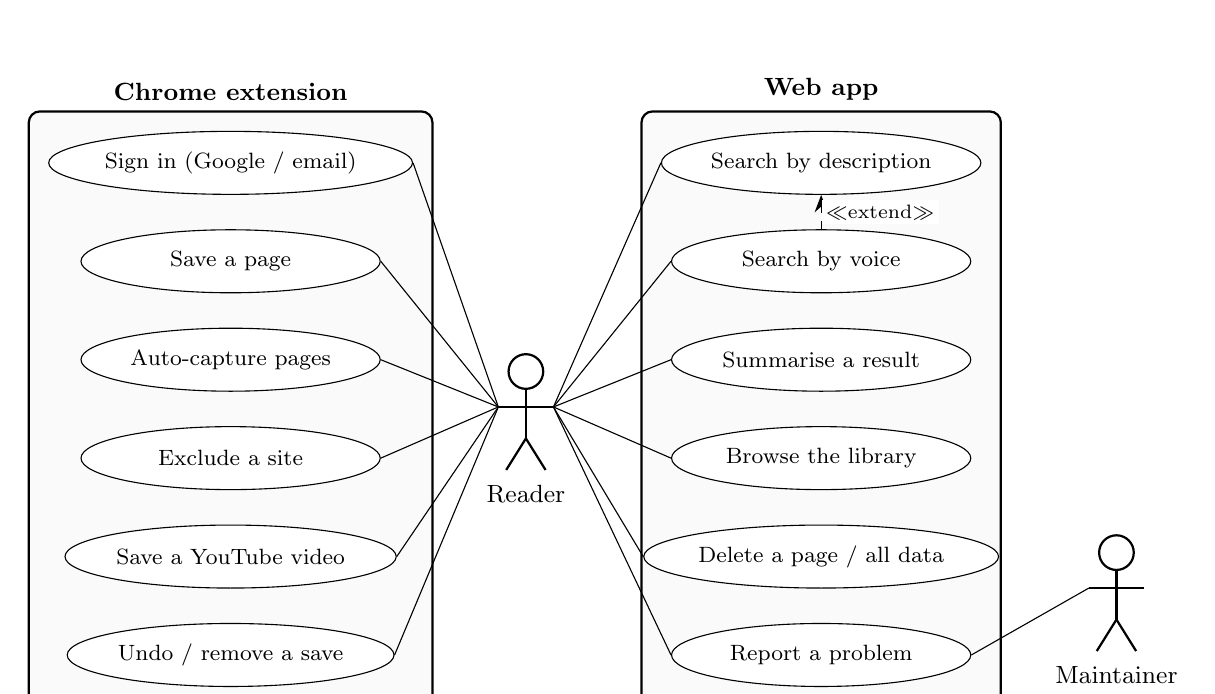
\begin{tikzpicture}[node distance=3mm]
  % stick figure: \actor{x}{y}{label}
  \newcommand{\actor}[3]{%
    \draw[thick] (#1,#2+0.45) circle (2.2mm);
    \draw[thick] (#1,#2+0.23) -- (#1,#2-0.4);
    \draw[thick] (#1-0.35,#2) -- (#1+0.35,#2);
    \draw[thick] (#1,#2-0.4) -- (#1-0.25,#2-0.8);
    \draw[thick] (#1,#2-0.4) -- (#1+0.25,#2-0.8);
    \node[font=\small] at (#1,#2-1.1) {#3};}
  \actor{0}{-3.1}{Reader}
  \actor{7.5}{-5.4}{Maintainer}

  % extension use cases (left) and web-app use cases (right)
  \tikzset{usecase/.append style={minimum width=38mm, minimum height=8mm, font=\footnotesize}}
  \node[usecase] (signin)  at (-3.75, 0.0)  {Sign in (Google / email)};
  \node[usecase] (save)    at (-3.75,-1.25) {Save a page};
  \node[usecase] (auto)    at (-3.75,-2.5)  {Auto-capture pages};
  \node[usecase] (exclude) at (-3.75,-3.75) {Exclude a site};
  \node[usecase] (yt)      at (-3.75,-5.0)  {Save a YouTube video};
  \node[usecase] (undo)    at (-3.75,-6.25) {Undo / remove a save};
  \node[usecase] (search)  at (3.75, 0.0)  {Search by description};
  \node[usecase] (voice)   at (3.75,-1.25) {Search by voice};
  \node[usecase] (summ)    at (3.75,-2.5)  {Summarise a result};
  \node[usecase] (lib)     at (3.75,-3.75) {Browse the library};
  \node[usecase] (del)     at (3.75,-5.0)  {Delete a page / all data};
  \node[usecase] (report)  at (3.75,-6.25) {Report a problem};

  \begin{scope}[on background layer]
    \node[group, fill=gray!4, fit=(signin)(undo), inner sep=7pt] (extbox) {};
    \node[group, fill=gray!4, fit=(search)(report), inner sep=7pt] (webbox) {};
  \end{scope}
  \node[font=\small\bfseries, anchor=south] at (extbox.north) {Chrome extension};
  \node[font=\small\bfseries, anchor=south] at (webbox.north) {Web app};

  \foreach \u in {signin,save,auto,exclude,yt,undo}
    \draw (-0.35,-3.1) -- (\u.east);
  \foreach \u in {search,voice,summ,lib,del,report}
    \draw (0.35,-3.1) -- (\u.west);
  \draw (7.15,-5.4) -- (report.east);
  \draw[dashed,->] (voice) -- node[lbl, right] {$\ll$extend$\gg$} (search);
\end{tikzpicture}
\caption{Use-case diagram of MemoryLane}
\label{fig:usecases}
\end{figure}

\section{Functional Requirements}

\begin{longtable}{>{\ttfamily}p{0.09\textwidth} p{0.6\textwidth} p{0.18\textwidth}}
\toprule
\textrm{\textbf{ID}} & \textbf{Requirement} & \textbf{Status} \\
\midrule
\endhead
FR-01 & Users sign in with Google or email and password; a Google and an email sign-in with the same verified email share one library. & Done \\
FR-02 & The extension saves the current page in one click, confirms it, and offers undo. & Done \\
FR-03 & Optional automatic capture saves only pages the user has read and that look like content, and never private pages (email, banking, private apps, account areas). & Done \\
FR-04 & Users can exclude sites from automatic capture and see and remove the day's automatic saves. & Done \\
FR-05 & YouTube videos are saved through their captions, with description and channel. & Done \\
FR-06 & Saving the same page again updates one entry; addresses that differ only in tracking parameters, \texttt{www.} or fragments are the same page. & Done \\
FR-07 & Users search with a natural-language description, by typing or by voice, and get up to ten pages with snippets. & Done \\
FR-08 & Queries that name a site, a time or a URL rank matching pages higher. & Done \\
FR-09 & Each result can be summarised on demand. & Done \\
FR-10 & Users browse their library newest first, delete pages with undo, and delete all their data. & Done \\
FR-11 & Users report a problem from the website or the extension; the report is emailed to the maintainer. & Done \\
FR-12 & A public health endpoint reports the state of Solr, the model and Gemini. & Done \\
\bottomrule
\caption{Functional requirements}
\label{tab:fr}
\end{longtable}

\section{Non-Functional Requirements}

\begin{table}[H]
\centering
\small
\begin{tabularx}{\textwidth}{>{\raggedright\arraybackslash}p{0.2\textwidth} L L}
\toprule
\textbf{Quality} & \textbf{Requirement} & \textbf{How it is met} \\
\midrule
Privacy & No user can see or change another user's pages; sensitive pages are never auto-saved; logs hold no URLs or queries & User filter inside the Solr client; isolation tests; two-stage capture rules; log filters \\
Security & Authenticated API; no secrets in the browser & Cognito PKCE, RS256 token checks, CSP, HTTPS with HSTS, rate limits \\
Performance & Search answers in well under a second & $\approx$75\,ms median in-process search; concurrent BM25 and KNN \\
Relevance & The right page is usually first & Hit@1 0.71, MRR@10 0.79 on SciFact (Chapter~\ref{ch:evaluation}) \\
Availability & Survives a reboot; degrades instead of failing & Restart policies, health checks; summaries and reports optional \\
Maintainability & Changes are safe and explained & 551 tests, CI, decision records, documentation site \\
Usability & Usable with keyboard and on phones & Keyboard shortcuts, responsive layout, voice input \\
Cost & Runs on one small server & One \texttt{c7i-flex.large} instance \\
\bottomrule
\end{tabularx}
\caption{Non-functional requirements}
\label{tab:nfr}
\end{table}

\section{Development Process}

MemoryLane was built \textbf{iteratively and incrementally}
\cite{sommerville2016se}: each iteration delivered a working system, which
was used, measured and then improved. Work was tracked in Git on GitHub, with
feature branches for larger changes (for example
\texttt{feature/library-map}) and 86 commits over four months.

\begin{figure}[H]
\centering
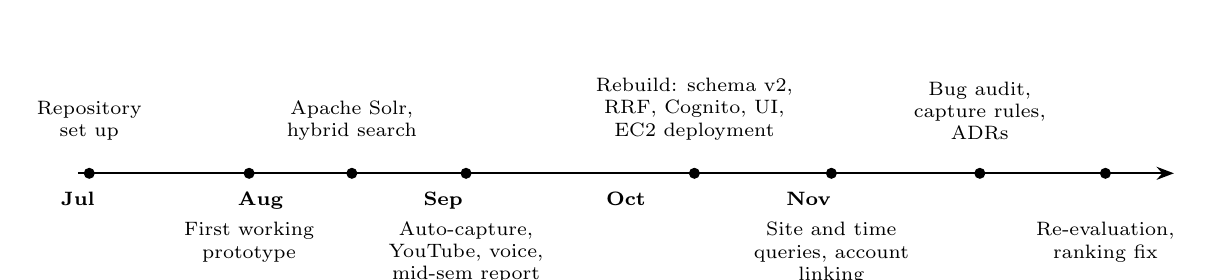
\begin{tikzpicture}[x=1.45cm]
  \draw[thick,->] (0,0) -- (9.6,0);
  \foreach \x/\m in {0/Jul, 1.6/Aug, 3.2/Sep, 4.8/Oct, 6.4/Nov}
    \node[font=\scriptsize\bfseries, below] at (\x,-0.12) {\m};
  \foreach \x in {0.1,1.5,2.4,3.4,5.4,6.6,7.9,9.0}
    \fill (\x,0) circle (2pt);
  \node[font=\scriptsize, align=center, above=3mm] at (0.1,0) {Repository\\ set up};
  \node[font=\scriptsize, align=center, below=5mm] at (1.5,0) {First working\\ prototype};
  \node[font=\scriptsize, align=center, above=3mm] at (2.4,0) {Apache Solr,\\ hybrid search};
  \node[font=\scriptsize, align=center, below=5mm] at (3.4,0) {Auto-capture,\\ YouTube, voice,\\ mid-sem report};
  \node[font=\scriptsize, align=center, above=3mm] at (5.4,0) {Rebuild: schema v2,\\ RRF, Cognito, UI,\\ EC2 deployment};
  \node[font=\scriptsize, align=center, below=5mm] at (6.6,0) {Site and time\\ queries, account\\ linking};
  \node[font=\scriptsize, align=center, above=3mm] at (7.9,0) {Bug audit,\\ capture rules,\\ ADRs};
  \node[font=\scriptsize, align=center, below=5mm] at (9.0,0) {Re-evaluation,\\ ranking fix};
\end{tikzpicture}
\caption{Project timeline, July--November 2026}
\label{fig:timeline}
\end{figure}

The October rebuild was planned as seven phases, each committed and tested
separately: query-side retrieval improvements, bug fixes, a new ingestion
pipeline and schema, authentication and multi-user scoping, a web redesign,
an extension redesign, and deployment with Docker Compose and Caddy. After
the system went live, real use drove the remaining work: an audit of
reported bugs, stricter automatic capture after an inbox was captured by an
outdated extension, and a second evaluation that uncovered a ranking defect
(Section~\ref{sec:bonus}).

Every significant choice was written down as an \textbf{architecture
decision record} (ADR) \cite{nygard2011adr}, giving the context, the
decision, the alternatives and the consequences (Table~\ref{tab:adrs}).
Features that did not earn their place were removed rather than kept, and
their removal was recorded too.

% ==================================================
% CHAPTER 3: SYSTEM DESIGN
% ==================================================

\chapter{System Design}
\label{ch:design}

\section{Architecture Overview}

MemoryLane has three client-facing parts and one server
(Figure~\ref{fig:architecture}). The \textbf{Chrome extension} captures
pages; the \textbf{web app} is where users search and manage their library;
and the \textbf{FastAPI backend} processes pages, runs searches and talks to
\textbf{Apache Solr}, which holds both the text index and the vectors. All
browser traffic enters through \textbf{Caddy}, which terminates HTTPS,
serves the built web app and proxies \texttt{/api/*} to the backend.

\begin{figure}[H]
\centering
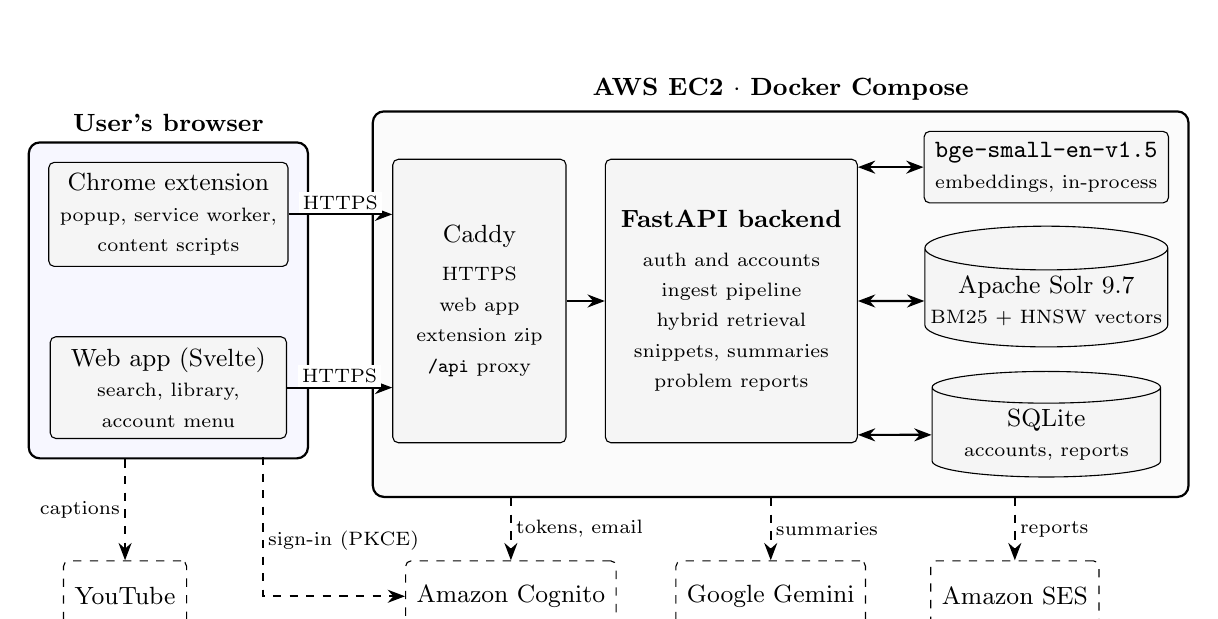
\begin{tikzpicture}
  % ---- browser -----------------------------------------------------------
  \node[comp, minimum width=30mm] (ext) at (0, 1.1) {Chrome extension\\\scriptsize popup, service worker,\\\scriptsize content scripts};
  \node[comp, minimum width=30mm] (web) at (0,-1.1) {Web app (Svelte)\\\scriptsize search, library,\\\scriptsize account menu};
  \begin{scope}[on background layer]
    \node[group, fill=blue!3, fit=(ext)(web), inner sep=7pt] (browser) {};
  \end{scope}
  \node[font=\small\bfseries, anchor=south] at (browser.north) {User's browser};

  % ---- server ------------------------------------------------------------
  \node[comp, minimum width=22mm, minimum height=36mm] (caddy) at (3.95, 0) {Caddy\\[1mm]\scriptsize HTTPS\\\scriptsize web app\\\scriptsize extension zip\\\scriptsize \texttt{/api} proxy};
  \node[comp, minimum width=32mm, minimum height=36mm] (api) at (7.15, 0)
    {\textbf{FastAPI backend}\\[1mm]\scriptsize auth and accounts\\\scriptsize ingest pipeline\\\scriptsize hybrid retrieval\\\scriptsize snippets, summaries\\\scriptsize problem reports};
  \node[comp, minimum width=29mm] (model) at (11.15, 1.7) {\texttt{bge-small-en-v1.5}\\\scriptsize embeddings, in-process};
  \node[db, minimum width=29mm] (solr)  at (11.15, 0)   {Apache Solr 9.7\\\scriptsize BM25 + HNSW vectors};
  \node[db, minimum width=29mm] (sqlite) at (11.15,-1.7) {SQLite\\\scriptsize accounts, reports};
  \begin{scope}[on background layer]
    \node[group, fill=gray!3, fit=(caddy)(api)(model)(sqlite), inner sep=7pt] (server) {};
  \end{scope}
  \node[font=\small\bfseries, anchor=south] at (server.north) {AWS EC2 $\cdot$ Docker Compose};

  % ---- external services ---------------------------------------------------
  \node[ext] (yt)      at (-0.55,-3.75) {YouTube};
  \node[ext] (cognito) at (4.35,  -3.75) {Amazon Cognito};
  \node[ext] (gemini)  at (7.65,  -3.75) {Google Gemini};
  \node[ext] (ses)     at (10.75, -3.75) {Amazon SES};

  % ---- flows ---------------------------------------------------------------
  \draw[flow] (ext.east) -- node[lbl, above] {HTTPS} (caddy.west |- ext.east);
  \draw[flow] (web.east) -- node[lbl, above] {HTTPS} (caddy.west |- web.east);
  \draw[flow] (caddy) -- (api);
  \draw[flow, <->] (api.east |- model) -- (model.west);
  \draw[flow, <->] (api.east |- solr) -- (solr.west);
  \draw[flow, <->] (api.east |- sqlite) -- (sqlite.west);
  \draw[flow, dashed] (yt.north |- browser.south) -- node[lbl, left] {captions} (yt.north);
  \draw[flow, dashed] (cognito.north |- server.south) -- node[lbl, right] {tokens, email} (cognito.north);
  \draw[flow, dashed] (gemini.north |- server.south) -- node[lbl, right] {summaries} (gemini.north);
  \draw[flow, dashed] (ses.north |- server.south) -- node[lbl, right] {reports} (ses.north);
  \draw[flow, dashed] (1.2,-1.98) |- node[lbl, pos=0.3, right] {sign-in (PKCE)} (cognito.west);
\end{tikzpicture}

\caption{Architecture of the deployed system. Dashed boxes are external services.}
\label{fig:architecture}
\end{figure}

The backend is a single process (one Uvicorn worker) that loads the
embedding model once and shares it between requests. Solr is the only
store for pages; two small SQLite databases hold sign-in links and problem
reports. The design keeps the number of moving parts small enough to run on
one server, a decision recorded in ADR~0004.

\section{Data Flow}

\subsection{Context Diagram (Level 0)}

\begin{figure}[H]
\centering
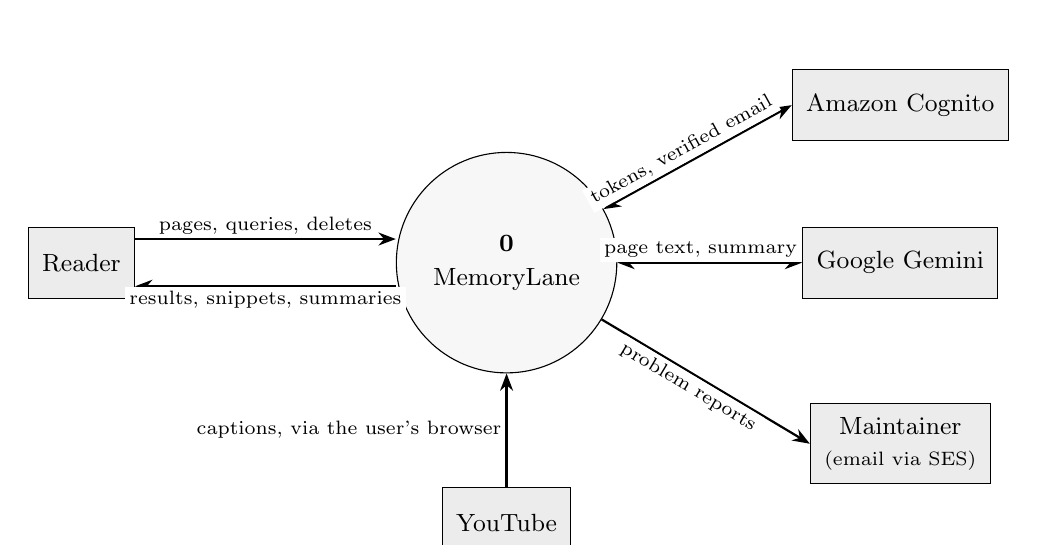
\begin{tikzpicture}
  \node[proc, minimum size=28mm] (ml) at (0,0) {\textbf{0}\\[0.5mm]MemoryLane};
  \node[entity] (user) at (-5.4, 0)   {Reader};
  \node[entity] (cog)  at (5.0, 2.0)  {Amazon Cognito};
  \node[entity] (gem)  at (5.0, 0)    {Google Gemini};
  \node[entity] (ses)  at (5.0,-2.3)  {Maintainer\\\scriptsize (email via SES)};
  \node[entity] (yt)   at (0,  -3.3)  {YouTube};

  \draw[flow] ([yshift=3mm]user.east) -- node[lbl, above] {pages, queries, deletes} ([yshift=3mm]ml.west);
  \draw[flow] ([yshift=-3mm]ml.west) -- node[lbl, below] {results, snippets, summaries} ([yshift=-3mm]user.east);
  \draw[flow, <->] (ml) -- node[lbl, above, sloped, pos=0.45] {tokens, verified email} (cog.west);
  \draw[flow, <->] (ml) -- node[lbl, above, pos=0.45] {page text, summary} (gem.west);
  \draw[flow] (ml) -- node[lbl, below, sloped, pos=0.45] {problem reports} (ses.west);
  \draw[flow] (yt) -- node[lbl, left] {captions, via the user's browser} (ml);
\end{tikzpicture}

\caption{Context data-flow diagram}
\label{fig:dfd0}
\end{figure}

\subsection{Level 1}

\begin{figure}[H]
\centering
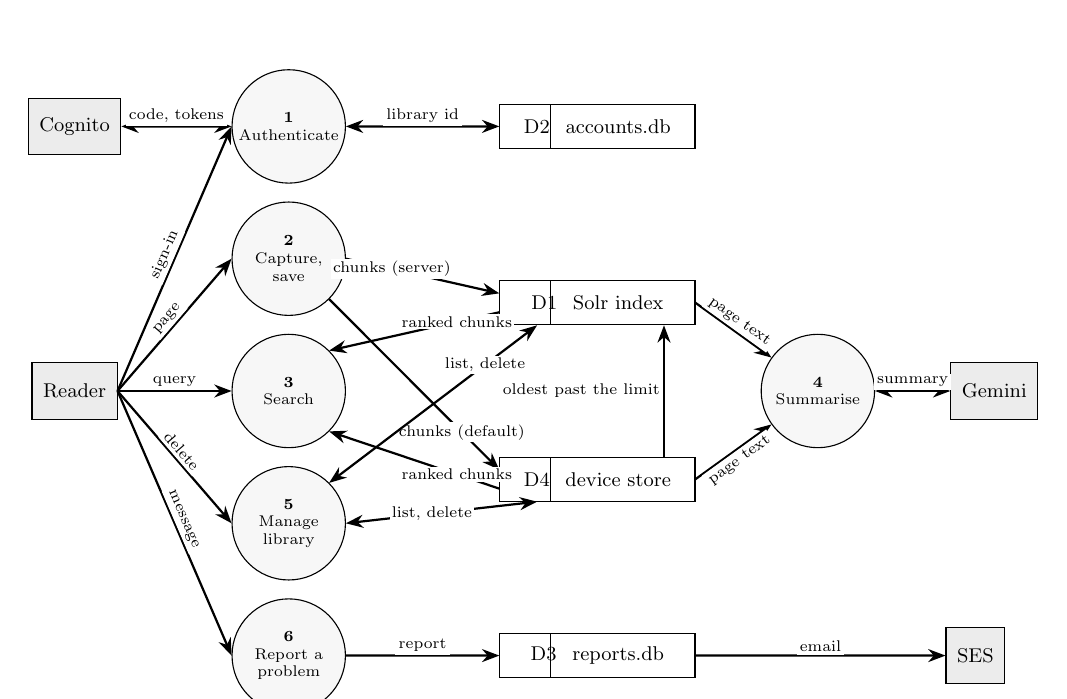
\begin{tikzpicture}[scale=0.8, transform shape, proc/.append style={minimum size=18mm, font=\scriptsize}]
  \newcommand{\dstore}[2]{\makebox[6.6mm][l]{#1}#2}
  \tikzset{wl/.style={lbl, fill=white, inner sep=1pt}}
  % external entities
  \node[entity] (user) at (-5.7, 0)   {Reader};
  \node[entity] (cog)  at (-5.7, 4.2) {Cognito};
  \node[entity] (gem)  at (8.9, 0)    {Gemini};
  \node[entity] (ses)  at (8.6,-4.2)  {SES};

  % processes
  \node[proc] (p1) at (-2.3, 4.2) {\textbf{1}\\Authenticate};
  \node[proc] (p2) at (-2.3, 2.1) {\textbf{2}\\Capture,\\save};
  \node[proc] (p3) at (-2.3, 0.0) {\textbf{3}\\Search};
  \node[proc] (p5) at (-2.3,-2.1) {\textbf{5}\\Manage\\library};
  \node[proc] (p6) at (-2.3,-4.2) {\textbf{6}\\Report a\\problem};
  \node[proc] (p4) at (6.1, 0)    {\textbf{4}\\Summarise};

  % data stores
  \node[store, minimum width=31mm] (d2) at (2.6, 4.2)  {\dstore{D2}{accounts.db}};
  \node[store, minimum width=31mm] (d1) at (2.6, 1.4)  {\dstore{D1}{Solr index}};
  \node[store, minimum width=31mm] (d4) at (2.6,-1.4)  {\dstore{D4}{device store}};
  \node[store, minimum width=31mm] (d3) at (2.6,-4.2)  {\dstore{D3}{reports.db}};

  % flows from the reader
  \foreach \p/\t in {p1/sign-in, p2/page, p3/query, p5/delete, p6/message}
    \draw[flow] (user.east) -- node[lbl, sloped, above, pos=0.5] {\t} (\p.west);

  \draw[flow, <->] (p1) -- node[lbl, above] {code, tokens} (cog);
  \draw[flow, <->] (p1) -- node[lbl, above] {library id} (d2);
  % capture writes to the device store (default) or to Solr
  \draw[flow] (p2.east) -- node[wl, pos=0.3] {chunks (server)} ([yshift=1.5mm]d1.west);
  \draw[flow] (p2.south east) -- node[wl, pos=0.78] {chunks (default)} ([yshift=1.5mm]d4.west);
  % search reads both stores
  \draw[flow] ([yshift=-1.5mm]d1.west) -- node[wl, pos=0.25] {ranked chunks} (p3.north east);
  \draw[flow] ([yshift=-1.5mm]d4.west) -- node[wl, pos=0.25] {ranked chunks} (p3.south east);
  % manage lists and deletes in both
  \draw[flow, <->] (p5.north east) -- node[wl, pos=0.75] {list, delete} ([xshift=6mm]d1.south west);
  \draw[flow, <->] (p5.east) -- node[wl, pos=0.45] {list, delete} ([xshift=6mm]d4.south west);
  % overflow and summaries
  \draw[flow] ([xshift=-5mm]d4.north east) -- node[lbl, left] {oldest past the limit} ([xshift=-5mm]d1.south east);
  \draw[flow] (d1.east) -- node[lbl, sloped, above] {page text} (p4);
  \draw[flow] (d4.east) -- node[lbl, sloped, below] {page text} (p4);
  \draw[flow, <->] (p4) -- node[lbl, above] {summary} (gem);
  \draw[flow] (p6) -- node[lbl, above] {report} (d3);
  \draw[flow] (d3) -- node[lbl, above] {email} (ses);
\end{tikzpicture}

\caption{Level-1 data-flow diagram}
\label{fig:dfd1}
\end{figure}

Every flow that touches D1 carries the verified library id of the caller;
there is no flow by which a client can name another user's id.

\section{Data Model}

\subsection{Pages and Chunks in Solr}

A saved page is stored as $n$ \emph{chunk documents} in one Solr core
(\texttt{memorylane\_v2}). Page-level fields are repeated on every chunk so
that a search hit needs no second lookup; chunk~0 additionally carries the
page vector. Table~\ref{tab:schema} lists the fields.

\begin{table}[H]
\centering
\small
\begin{tabularx}{\textwidth}{>{\ttfamily}p{0.25\textwidth} p{0.2\textwidth} L}
\toprule
\textrm{\textbf{Field}} & \textbf{Type} & \textbf{Purpose} \\
\midrule
id & string & \texttt{\{page\_id\}::\{chunk\_id\}}, so re-saving overwrites in place \\
user\_id & string & Owner's library id; on every query as a filter \\
page\_id & string & \texttt{sha256(user\_id|normalised URL)[:32]} \\
url, domain & string & Normalised address and host \\
title & text\_en & Page title (weighted $\times 2$ in BM25) \\
text & text\_en & The chunk's passage (stemmed, stop-words removed) \\
description & stored & Meta description or first sentences; snippet fallback \\
chunk\_id, total\_chunks & int & Position of the chunk, chunks in the page \\
timestamp & date & When the page was saved \\
content\_hash & string & SHA-256 of the cleaned text; skips unchanged re-saves \\
embedding\_model & string & Model that produced the vectors; a change forces re-embedding \\
embedding & vector(384) & Chunk vector, cosine, HNSW index \\
page\_embedding & vector(384) & Mean of the chunk vectors (chunk~0 only) \\
\bottomrule
\end{tabularx}
\caption{Solr schema (\texttt{schema v2})}
\label{tab:schema}
\end{table}

Automatic field creation is turned off, so a field must be added by a
script before code that writes it is deployed.

\subsection{Relational Data}

Two SQLite databases live in a Docker volume next to Solr's data:

\begin{itemize}
  \item \texttt{accounts.db}: which Cognito sign-ins (\texttt{sub}) share a
  library, the verified email that links them, when each was last checked
  with Cognito, and libraries waiting to be merged after a late
  verification.
  \item \texttt{reports.db}: problem reports and their email delivery
  state, so that a report is never lost when email is temporarily failing
  (ADR~0007).
\end{itemize}

\section{Interface Design}

\subsection{REST API}

\begin{table}[H]
\centering
\small
\begin{tabularx}{\textwidth}{>{\ttfamily}p{0.11\textwidth} >{\ttfamily}p{0.27\textwidth} L r}
\toprule
\textrm{\textbf{Method}} & \textrm{\textbf{Endpoint}} & \textbf{Purpose} & \textbf{Limit} \\
\midrule
GET & /health & Public status of Solr, model, Gemini & -- \\
POST & /memory & Save or update a page & 60/min \\
GET & /memory/status & Is this URL saved? & 120/min \\
POST & /memory/existing & Which of these pages still exist? & 120/min \\
DELETE & /memory/\{id\} & Delete one page & 60/min \\
GET & /memory/\{id\}/related & Pages closest in meaning & 120/min \\
GET & /memories & Library, newest first & 60/min \\
POST & /search & Hybrid search & 60/min \\
POST & /summarize & Summary of one page & 20/min \\
DELETE & /me/data & Delete all the caller's data & 5/min \\
POST & /reports & Report a problem & 5/hour \\
\bottomrule
\end{tabularx}
\caption{API endpoints. All except \texttt{/health} need a Cognito access token.}
\label{tab:api}
\end{table}

\subsection{User Interface}

The web app is deliberately quiet: a dark theme, one search box, and results
that show the title, site, save time and a highlighted snippet. Every action
has a keyboard path (\texttt{/} to search, arrows to move, \texttt{S} to
summarise, \texttt{Shift+Del} to delete with undo). The extension popup
shows whether the current page is saved, one primary button, and the day's
automatic saves with one-click removal.

\section{Design Decisions}

Table~\ref{tab:adrs} lists the architecture decision records kept with the
code. Each record states the alternatives that were rejected and the cost of
the choice.

\begin{table}[H]
\centering
\small
\begin{tabularx}{\textwidth}{>{\ttfamily}p{0.06\textwidth} p{0.36\textwidth} L}
\toprule
\textrm{\textbf{\#}} & \textbf{Decision} & \textbf{Main reason} \\
\midrule
0001 & One Solr core for keyword and vector search & One system for BM25, KNN and filters; no second database to keep in sync \\
0002 & Fuse rankings with Reciprocal Rank Fusion & Rank-based, so no score normalisation and no outlier effects \\
0003 & Drop weak matches with a relevance floor & KNN always returns neighbours, however unrelated \\
0004 & Run everything on one EC2 instance & Cost and simplicity at this scale \\
0005 & Link sign-ins by verified email & One library per person, without trusting the browser \\
0006 & Fetch YouTube captions in the browser & YouTube blocks requests from servers \\
0007 & Store problem reports before emailing & A report survives an email outage \\
0008 & Keep summaries on demand and optional & Search never waits on an external model \\
0009 & Remove the library map & Costly, fragile and rarely useful \\
0010 & Remove ``Export my data'' & Little use; deleting data is the stronger right \\
0011 & Auto-capture keeps only pages that read like content & Rules on content and reading, not an endless site list \\
\bottomrule
\end{tabularx}
\caption{Architecture decision records}
\label{tab:adrs}
\end{table}

% ==================================================
% CHAPTER 4: IMPLEMENTATION
% ==================================================

\chapter{Implementation}
\label{ch:implementation}

\section{Code Base}

The repository holds the backend (23 Python modules, about 4{,}000 lines), the web app (21 Svelte components), the Chrome extension, 551 tests, the evaluation scripts and the documentation. Table~\ref{tab:modules} lists the main backend modules.

\begin{table}[!htbp]
\centering
\small
\begin{tabularx}{\textwidth}{>{\ttfamily}p{0.25\textwidth} L}
\toprule
\textrm{\textbf{Module}} & \textbf{Responsibility} \\
\midrule
main.py & API endpoints, rate limits, log filtering, automatic-save re-check \\
auth.py, accounts.py & Token verification; linking sign-ins by verified email \\
library\_moves.py & Background merge of a library into the linked one \\
ingest.py & The save pipeline, under a per-user write lock \\
cleaning.py, chunking.py & Main-content extraction; overlapping chunks \\
embeddings.py & Model loading, batched passage and cached query embedding \\
retrieval.py & BM25 + KNN, fusion, page grouping, relevance floor \\
query\_intent.py & Site words, time phrases and URLs in queries \\
snippets.py & Sentence snippets for each result \\
solr\_client.py & All Solr access, with the user filter built in \\
page\_filter.py & Rules for pages automatic capture must refuse \\
summarizer.py & On-demand Gemini summaries with a time limit \\
reports.py & Stored problem reports and the email sender \\
youtube\_utils.py & Validated video ids and transcript processing \\
\bottomrule
\end{tabularx}
\caption{Main backend modules}
\label{tab:modules}
\end{table}

\section{Browser Extension}

The extension is a Manifest V3 extension \cite{chromemv3} with a popup, a
background service worker and scripts injected into pages only when needed.
It signs in through Cognito with \texttt{chrome.identity} and keeps its
tokens in \texttt{chrome.storage.local}, which web pages cannot read.

\subsection{Saving a Page}

\textbf{Remember this page} injects a content script that returns the page's
HTML, its visible text and its canonical URL. Single-page applications such
as Reddit and YouTube change the address without reloading and keep a stale
canonical tag, so a canonical URL is sent only when it describes the current
page (same host and path, and matching parameters). The popup confirms the
save and offers \textbf{Undo}.

\subsection{YouTube}

YouTube refuses transcript requests from servers. For a video, the
extension therefore fetches the caption track, title, channel, length and
description \emph{inside the user's own tab}, and sends them with the save
(ADR~0006). A video without captions is saved from its description.

\subsection{Automatic Capture}

Automatic capture is off by default and explained before it is turned on.
Rather than trying to list every site that should not be saved, it keeps a
page only if it passes three tests (swimlane diagram, Figure~\ref{fig:swimlane}):

\begin{enumerate}
  \item \textbf{The address is not private}: not email, banking, social
  media, a private application (documents, chat, cloud consoles, college
  portals), a local address, an account area, or a link carrying a secret.
  \item \textbf{The user read it}: the page was visible for 30 seconds, or
  scrolled at least halfway after 5 seconds. Pages bounced off are never
  saved.
  \item \textbf{It reads like content}: at least 150 readable words, not
  mostly links, no visible password field, no large editor or form, and not
  marked \texttt{noindex}.
\end{enumerate}

The same address rules are applied again by the server to every automatic
save, so even an outdated or faulty extension cannot store an inbox or a
login page. An automatic save never rewrites a page that is already in the
library; only a manual save updates one. The popup lists the day's automatic
saves with \textbf{Remove} and \textbf{Never this site}, and drops entries the
user has since deleted on the website.

\begin{figure}[!htbp]
\centering
\begin{subfigure}[b]{0.52\textwidth}
  \centering
  \screenshot[\textwidth]{figures/extension-popup.png}{extension popup}
  \caption{Popup after a save, with ``Auto-saved today''}
\end{subfigure}\hfill
\begin{subfigure}[b]{0.44\textwidth}
  \centering
  \screenshot[\textwidth]{figures/excluded-sites.png}{excluded sites page}
  \caption{Excluded sites (options page)}
\end{subfigure}
\caption{The Chrome extension}
\label{fig:extension}
\end{figure}

\section{Ingestion Pipeline}

All saves, from the API, the re-index scripts and the evaluation, go through
one function, \texttt{ingest\_page} (Figure~\ref{fig:seq-save}). Writes for one
user run under that user's lock, so two saves cannot race on the page
limit or leave duplicate chunks.

\subsection{URL Normalisation and Identity}

The same page can have many addresses. Normalisation lower-cases the scheme
and host, removes \texttt{www.}, fragments, trailing slashes and tracking
parameters (\texttt{utm\_*}, \texttt{fbclid}, \texttt{gclid}, \texttt{ref}),
and sorts the remaining parameters. The page id is

\[
\texttt{page\_id} = \mathrm{SHA256}(\texttt{user\_id} \,\|\, \texttt{"|"} \,\|\, \textit{normalised URL})_{[0:32]},
\]

so the same page saved twice updates one entry, and two users' copies of a
page can never collide.

\subsection{Cleaning and Chunking}

trafilatura \cite{barbaresi2021trafilatura} extracts the main text of the
HTML and drops navigation, footers and banners; if it finds too little, the
extension's visible text is used. Citation markers and junk lines are then
removed. The text is split into paragraphs and sentences and packed into
chunks of at most 150 words, each starting with about 30 words from the end
of the previous chunk, so an idea is never cut in half at a boundary. A
short final chunk merges into the one before.

\subsection{Embeddings}

Each chunk is embedded as ``title + chunk'' with \texttt{BAAI/bge-small-en-v1.5}
\cite{xiao2023bge} through Sentence Transformers \cite{reimers2019sbert}:
384-dimensional, L2-normalised vectors, computed in batches of 32 on the CPU.
Queries are embedded with BGE's retrieval instruction in front, and the last
1{,}024 query vectors are cached. A content hash and the model name are
stored with each page, so an unchanged page costs one lookup to re-save, and
a model change re-embeds pages the next time they are saved.

\section{Hybrid Retrieval}

Figures~\ref{fig:seq-search} and~\ref{fig:collab-search} show one search from query to results, and Figure~\ref{fig:dfd2} its data flow.

\subsection{Lexical and Semantic Retrieval}

BM25 \cite{robertson2009bm25} runs through Solr's edismax parser over
\texttt{title\^{}2 text}, with a phrase boost so pages containing the query as
a phrase rank higher, and with field syntax in user input disabled. The
query vector is searched with Solr's HNSW KNN \cite{solr}, using the user
filter as a \emph{pre-filter} so all 50 neighbours belong to the caller. The
two run concurrently.

\subsection{Site, Time and URL in the Query}

People often remember \emph{where} or \emph{when} they saw something. The
query-intent module recognises:

\begin{itemize}
  \item \textbf{site words}: names derived from the domains the user has
  actually saved (\texttt{en.wikipedia.org} $\rightarrow$ \textit{wikipedia},
  \texttt{docs.nvidia.com} $\rightarrow$ \textit{nvidia}), joined words
  (\textit{rotten tomatoes}) and a few nicknames (\textit{yt}, \textit{gh});
  \item \textbf{time phrases}: \textit{yesterday}, \textit{3 weeks ago},
  \textit{last month}, \textit{in march}, \textit{31 august}, \textit{recently};
  \item \textbf{a URL or domain} as the whole query.
\end{itemize}

When one is found, the rest of the query is searched again within those
domains and dates, and the extra lists join the fusion as boosts rather than
filters, so a better page from elsewhere still wins.

\subsection{Reciprocal Rank Fusion}

BM25 scores and cosine similarities live on different scales. The prototype
min-max normalised and averaged them, which lets one outlier shift every
other score. The final system fuses \emph{ranks} with Reciprocal Rank Fusion
\cite{cormack2009rrf} (ADR~0002):

\[
\mathrm{RRF}(d) \;=\; \sum_{\ell \,\in\, \text{lists}} \frac{w_\ell}{k + r_\ell(d)},
\qquad k = 60,\; w_\ell = 1,
\]

where $r_\ell(d)$ is the rank of chunk $d$ in list $\ell$, and a chunk
missing from a list gets nothing from it. Chunks found by both retrievers
rise to the top.

\subsection{Page Grouping and the Relevance Floor}

Users see pages, not chunks. Each page is scored by its best chunk,
$S_{\text{page}} = s_{\text{best}}$; Section~\ref{sec:bonus} explains why an
earlier bonus for a second matching chunk was removed. KNN always returns
neighbours, however unrelated, so a page found only by meaning is kept only
if its best cosine similarity is at least $0.55$ (ADR~0003). A page found by
keywords must hold at least 75\% of the query's words, or else meet the same
similarity bar: BM25 accepts a page that shares any single word, and for
``greatest football player of all time'' that would otherwise admit the
Nintendo article (``the greatest games of all time'').

\subsection{Snippets}

For each result, two or three consecutive readable sentences around the
sentence with the most query terms are shown, with the terms highlighted.
When no sentence shares a term (a search by meaning), the first readable
sentences are compared with the query by embedding instead.

\section{Summaries}

\textbf{Summarise} on a result asks Google Gemini \cite{gemini} for a short
summary of that page, adapted to the query, with a 20-second limit. Summaries
are on demand only, so search never waits on an external model, and the
system works fully without a Gemini key (ADR~0008).

\section{Web Application}

The web app is a Svelte \cite{svelte} single-page application served by
Caddy. Figure~\ref{fig:webapp} shows its main screens.

\begin{figure}[!htbp]
\centering
\begin{subfigure}[b]{\textwidth}
  \centering
  \screenshot[0.92\textwidth]{figures/search-results.png}{search results}
  \caption{A search naming a site (``nvidia docs on cuda graphs''): the matching
  snippet with query words highlighted, and the page's summary opened}
\end{subfigure}

\vspace{4mm}
\begin{subfigure}[b]{\textwidth}
  \centering
  \screenshot[0.7\textwidth]{figures/library.png}{library}
  \caption{The library, newest first (a delete button appears on each row on hover)}
\end{subfigure}
\caption{The web application}
\label{fig:webapp}
\end{figure}

Deleting is optimistic: the page disappears at once and a toast offers
\textbf{Undo} for six seconds before the request is sent. If the tab is
closed or reloaded in that window, the delete is sent immediately and the
reloaded page keeps it hidden. Voice search uses the browser's speech
recognition to fill the search box.

\section{Problem Reports}

\textbf{Report a problem}, on the website and in the extension, shows the
user exactly what will be sent (message, app version, page, browser, last
error) and stores the report in SQLite before a background sender emails it
through Amazon SES with retries (ADR~0007).

\section{Documentation Site}

The documentation is a 48-page MkDocs Material \cite{mkdocsmaterial} site
published on GitHub Pages, with a user guide, architecture and data-flow
diagrams, the API reference, the evaluation, the decision records and a
glossary. Its search box finds sections \emph{by meaning} as well as by
keywords, using the same idea as MemoryLane itself at a smaller scale: at
build time every section is embedded with the static model Model2Vec
\texttt{potion-base-8M} \cite{model2vec}, and in the browser a query is
tokenised, averaged into a vector and compared with all sections in a few
milliseconds, with no neural network running. The results are fused with the
keyword results by RRF. The files (about 8\,MB) load only when the search box
is first focused.

% ==================================================
% CHAPTER 5: SECURITY AND PRIVACY
% ==================================================

\chapter{Security and Privacy}
\label{ch:security}

MemoryLane stores what people read, which can be personal. Its main security
property is \textbf{isolation}: nobody can read, search, summarise or delete
another person's pages. Its main privacy property is \textbf{restraint}: it
does not collect what it should not.

\section{Authentication}

Sign-in is handled by Amazon Cognito \cite{cognito}, with Google or email
and password; MemoryLane never handles a password. The web app and the
extension use the OAuth 2.0 authorization-code flow \cite{rfc6749} with PKCE
\cite{rfc7636} and a public client, so no client secret ships to the
browser.

\begin{figure}[!htbp]
\centering
\begin{tikzpicture}[x=3.05cm, y=0.5cm]
  \foreach \i/\t in {0/{User}, 1/{:Web app}, 2/{:Amazon\\Cognito}, 3/{:FastAPI}, 4/{:accounts.db}} {
    \node[lifehead] (h\i) at (\i,0) {\t};
    \draw[life] (h\i.south) -- (\i,-19.0);
  }
  \newcommand{\m}[4]{\draw[msg] (#1,#3) -- node[mlabel, fill=white] {#4} (#2,#3);}
  \newcommand{\rt}[4]{\draw[ret] (#1,#3) -- node[mlabel, fill=white] {#4} (#2,#3);}
  \newcommand{\self}[3]{\draw[msg] (#1,#2) -- ++(0.1,0) -- ++(0,-0.75) node[font=\scriptsize, right, pos=0.5, align=left, fill=white, inner sep=1pt] {#3} -- ++(-0.1,0);}

  \m{0}{1}{-1.6}{Sign in}
  \self{1}{-2.2}{make verifier and\\SHA-256 challenge}
  \m{1}{2}{-3.9}{/oauth2/authorize (challenge)}
  \m{2}{0}{-4.8}{hosted sign-in (Google or email)}
  \m{0}{2}{-5.7}{credentials}
  \rt{2}{1}{-6.6}{redirect with one-time code}
  \m{1}{2}{-7.5}{/oauth2/token (code + verifier)}
  \rt{2}{1}{-8.4}{access + refresh tokens}
  \m{1}{3}{-9.5}{API request, Bearer access token}
  \self{3}{-10.1}{verify RS256, exp,\\iss, token\_use, client\_id}
  \m{3}{4}{-11.8}{library for this sub?}
  % alt frame
  \draw (2.55,-12.4) rectangle (4.35,-17.6);
  \node[draw, fill=white, font=\tiny, anchor=north west, inner sep=1.5pt] at (2.55,-12.4) {alt};
  \node[font=\tiny, anchor=west] at (2.6,-12.95) {[known sign-in]};
  \rt{4}{3}{-13.5}{library id}
  \draw[densely dashed] (2.55,-14.1) -- (4.35,-14.1);
  \node[font=\tiny, anchor=east] at (4.3,-14.55) {[first time]};
  \m{3}{2}{-15.2}{/oauth2/userInfo (user's token)}
  \rt{2}{3}{-16.0}{email, email\_verified}
  \m{3}{4}{-16.9}{link sub to library of verified email}
  \rt{3}{1}{-18.4}{response (only that library's data)}
\end{tikzpicture}

\caption{Sequence diagram: sign-in (authorization code with PKCE) and the first API request}
\label{fig:seq-signin}
\end{figure}

The access token is kept only in memory and the refresh token in local
storage, so a reload stays signed in. Because a script on the page could read
that token, the app never renders user-supplied HTML, and Caddy sends a
strict Content Security Policy. The session ends only when Cognito actually
refuses the refresh token; a refresh cancelled by a reload, a network error
or throttling keeps the user signed in.

\section{One Library per Person}

Cognito gives a Google sign-in and an email sign-in different identifiers
even for the same address. The backend links them by \emph{verified} email
(ADR~0005): the first time an identifier is seen, it asks Cognito for the
email using the user's own token, so the browser cannot fake it. An
unverified sign-in keeps a separate library until it is verified, and its
pages are then moved across in the background. Links are re-checked daily,
and if Cognito cannot be reached for a new identifier the request fails
rather than guessing.

\section{Data Isolation}

Isolation is enforced in the data-access layer, not left to each endpoint:

\begin{itemize}
  \item The Solr client adds the caller's library filter to \emph{every}
  query, scan, KNN search and delete, and refuses to run without a valid id.
  \item KNN uses the filter as a pre-filter, so other users' vectors are
  never even candidates.
  \item The user id is part of every page id, so copies never collide.
  \item A request for another user's page returns \texttt{404}, exactly like
  a missing page, so ids cannot be probed.
  \item No endpoint accepts a user id from the client.
\end{itemize}

\section{Threat Model}

Table~\ref{tab:threats} relates the main threats, several from the OWASP
Top~10 \cite{owasp2021}, to their mitigations.

\begin{table}[!htbp]
\centering
\small
\begin{tabularx}{\textwidth}{p{0.27\textwidth} L}
\toprule
\textbf{Threat} & \textbf{Mitigation} \\
\midrule
Reading another user's pages (broken access control) & Library filter in the Solr client; pre-filtered KNN; 404 for foreign ids; isolation tests \\
Forged or replayed tokens & RS256 verification against Cognito's keys; expiry, issuer, token type and client checks \\
Stolen refresh token via injected script (XSS) & No user HTML rendered; strict CSP; tokens out of reach of pages in the extension \\
Query injection into Solr & Field syntax disabled; values escaped; ids validated \\
Server-side request forgery & The backend never fetches a client-supplied URL \\
Abuse and resource exhaustion & Per-user rate limits; 5{,}000-page cap; request size limits \\
Sensitive pages captured & Address, reading and content rules; server re-check; one-click removal \\
Personal data in logs & Query strings dropped from access logs; Solr and Cognito request URLs not logged \\
Exposed internals & Only ports 80/443 open; Solr bound to localhost; backend unpublished \\
\bottomrule
\end{tabularx}
\caption{Threats and mitigations}
\label{tab:threats}
\end{table}

\section{Privacy}

Automatic capture is off by default and never captures private pages
(Figure~\ref{fig:swimlane}). Logs hold page ids, never the URLs people save
or what they search for, and a test checks it. Page text leaves the server
only when the user asks for a summary of that page, and users can delete any
page, or all their data, at any time.

% ==================================================
% CHAPTER 6: TESTING AND QUALITY ASSURANCE
% ==================================================

\chapter{Testing and Quality Assurance}
\label{ch:testing}

\section{Strategy}

Testing works at four levels \cite{pressman2014se}:

\begin{enumerate}
  \item \textbf{Unit tests} for pure logic: URL normalisation, cleaning,
  chunking, fusion, query intent, snippets, the capture rules, the delete
  queue and the docs-search tokenizer.
  \item \textbf{Integration tests} of the API through FastAPI's test client,
  with an in-memory stand-in for Solr that honours the user filter, and
  mocked Cognito, Gemini and SMTP.
  \item \textbf{System evaluation} against a real Solr instance with the
  production search code (Chapter~\ref{ch:evaluation}).
  \item \textbf{Manual verification} of the user interface in a browser,
  and on the live site after each deployment.
\end{enumerate}

Every bug fixed after launch got a regression test that fails without the
fix.

\section{Automated Test Suites}

\begin{table}[H]
\centering
\small
\begin{tabularx}{\textwidth}{p{0.36\textwidth} L r}
\toprule
\textbf{Area} & \textbf{What is checked} & \textbf{Tests} \\
\midrule
\multicolumn{3}{l}{\textit{Backend (pytest)}} \\
Query intent & Site words, time phrases, URLs, edge cases & 46 \\
Ingestion & Save, unchanged, update without duplicate chunks, limits, races & 45 \\
API & Endpoints, validation, errors, log privacy & 42 \\
Snippets & Sentence choice, highlighting, fallbacks & 37 \\
Solr client & User filter on every call, escaping, commits & 35 \\
Accounts and auth & Linking, re-checks, moves; token checks, 401 vs 503 & 45 \\
Retrieval and rerank & Fusion, grouping, floor, keyword coverage & 27 \\
Reports & Storage, sending, retries & 20 \\
Capture rules & Email, private apps, secrets, server refusal & 19 \\
Isolation & Two users: search, status, delete, library, related & 11 \\
Content & Cleaning, chunking, URLs, YouTube & 50 \\
Audit, evaluation, scripts & Bug-audit regressions, metrics, backfill, re-index & 38 \\
\midrule
\multicolumn{3}{l}{\textit{Frontend and extension (Vitest)}} \\
Extension rules & Capture rules identical to the backend's; domains & 76 \\
Delete queue & Undo, flush on close, restore after reload, reconcile & 15 \\
Docs search & Browser tokenizer and vectors equal the build's & 15 \\
Sessions, reports, misc. & Sign-in refresh, YouTube parsing, report form & 30 \\
\midrule
\textbf{Total} & & \textbf{551} \\
\bottomrule
\end{tabularx}
\caption{Automated tests by area (415 backend, 136 frontend)}
\label{tab:tests}
\end{table}

\subsection{Testing Isolation}

\texttt{test\_isolation.py} creates two users who save the same URL and then
tries every way user~A could reach user~B's page: searching for it,
summarising it, deleting it, checking its status, listing the library,
fetching related pages and deleting all data. It also checks that every
request the Solr client sends carries the user filter.

\subsection{Continuous Checks}

A GitHub Actions workflow builds the documentation in strict mode on every
push that touches it, so a broken link or diagram fails the check. The
frontend is type-checked with \texttt{svelte-check}, and its production
build is part of the Docker image, so a build error stops a deployment.

\section{Defects Found and Fixed}

Real use surfaced defects that unit tests alone had missed. A structured bug
audit in November and later reports were triaged, fixed with regression
tests, and documented. Table~\ref{tab:bugs} lists representative ones.

\begin{table}[H]
\centering
\small
\begin{tabularx}{\textwidth}{p{0.27\textwidth} L L}
\toprule
\textbf{Symptom} & \textbf{Root cause} & \textbf{Fix} \\
\midrule
An email inbox was auto-captured & An outdated extension, and a server that trusted it & Content-based rules; server re-checks every automatic save \\
Reddit posts collapsed into one saved page & Single-page apps keep a stale canonical tag & Canonical used only if it matches the current page \\
Rapid reloads signed the user out & A refresh cancelled by the reload was treated as a refused token & Sign out only when Cognito refuses; unreachable keys give 503 \\
A deleted page came back after a reload & The reload's list arrived before the delete was committed & Soft commit on delete; reloaded tab re-sends flushed deletes \\
Auto-capture re-dated an already-saved page & Slightly different extracted text counted as a change & Automatic saves never rewrite a saved page \\
Deleted pages stayed in ``Auto-saved today'' & The list lived only in the extension & Popup asks the server which pages still exist \\
Search text and user ids in server logs & The HTTP client logged every Solr request URL & Quietened those loggers; test proves no leak \\
Longer pages outranked better matches & Second-chunk bonus larger than RRF rank gaps & Score pages by their best chunk (Section~\ref{sec:bonus}) \\
\bottomrule
\end{tabularx}
\caption{Representative defects and their fixes}
\label{tab:bugs}
\end{table}

The last of these was found not by a user but by the evaluation, which is
the strongest argument for measuring retrieval quality rather than judging it
by eye.

% ==================================================
% CHAPTER 7: EVALUATION
% ==================================================

\chapter{Retrieval Evaluation}
\label{ch:evaluation}

\section{Benchmark}

Retrieval is evaluated on \textbf{SciFact} \cite{wadden2020scifact}, a
scientific-claim retrieval task from the BEIR benchmark
\cite{thakur2021beir}, adapted to MemoryLane's data model:

\begin{itemize}
  \item 1{,}000 SciFact abstracts saved as pages, each with a synthetic
  address of the form \path{https://scifact.org/doc/{id}}; 999 were indexed
  (one abstract fails cleaning and is not the answer to any claim);
  \item 100 claims as queries, with 115 claim--abstract relevance pairs.
\end{itemize}

The benchmark uses the production code end to end: abstracts are saved
through \texttt{ingest\_page} (cleaning, chunking, embedding, indexing) and
queries go through \texttt{hybrid\_search}, the function behind
\texttt{POST /search}. Everything runs in a separate Solr core under a
dedicated user id, so benchmark data never mixes with real libraries. The
final runs used a throwaway Solr 9.7 container on a laptop.

\section{Metrics}

The prototype reported three metrics. The final evaluation reports seven
quality metrics, two behaviour metrics, latency, and confidence intervals.
With $Q$ the claims, $\text{rel}_q$ the relevant abstracts of claim $q$, and
$r_q$ the rank of its first relevant result:

\begin{align*}
\text{Hit@}k &= \frac{1}{|Q|}\sum_{q} \mathbf{1}[r_q \leq k],
\qquad\qquad
\text{MRR@10} = \frac{1}{|Q|}\sum_{q} \frac{\mathbf{1}[r_q \le 10]}{r_q}, \\[2mm]
\text{Recall@10} &= \frac{1}{|Q|}\sum_{q} \frac{|\text{top}_{10}(q) \cap \text{rel}_q|}{|\text{rel}_q|}, \\[2mm]
\text{nDCG@10} &= \frac{1}{|Q|}\sum_{q}\frac{\sum_{i \le 10} \mathbf{1}[d_i \in \text{rel}_q]\,/\log_2(i+1)}{\sum_{i \le \min(10,|\text{rel}_q|)} 1/\log_2(i+1)},
\end{align*}

and MAP@10, the mean over claims of the precision at each relevant result in
the top ten \cite{manning2008ir,jarvelin2002ndcg}. In plain terms:

\begin{table}[H]
\centering
\small
\begin{tabularx}{\textwidth}{p{0.24\textwidth} L}
\toprule
\textbf{Metric} & \textbf{Meaning} \\
\midrule
Hit@1, Hit@3, Hit@10 & Share of claims with a right abstract first, in the top 3, in the top 10 \\
MRR@10 & How high the first right abstract is (1 = always first, 0.5 = second on average) \\
Recall@10 & Share of all right abstracts that appear in the top ten \\
nDCG@10, MAP@10 & How well all right abstracts are ordered, mistakes near the top counting most \\
Empty rate & Share of claims with no results at all (what the relevance floor could cause) \\
Latency p50 / p95 & In-process search time: the middle case and the slowest 5\% \\
95\% interval & Bootstrap range of Hit@1 and MRR@10 (2{,}000 resamples of the claims) \cite{efron1993bootstrap} \\
\bottomrule
\end{tabularx}
\caption{Evaluation metrics}
\label{tab:metrics}
\end{table}

Before timing, every claim is searched once untimed so no configuration
pays for cold caches, and each configuration starts with an empty query
cache.

\section{Configurations}

Five configurations were run, each by changing one setting for that run
only: \textbf{Hybrid} (the live search), \textbf{BM25 only},
\textbf{Vector only}, \textbf{Hybrid without the relevance floor}, and
\textbf{Hybrid with the old second-chunk bonus} (0.3).

\section{Results}

\begin{table}[H]
\centering
\small
\setlength{\tabcolsep}{2.4pt}
\begin{tabular}{lccccccc}
\toprule
\textbf{Configuration} & \textbf{Hit@1} & \textbf{Hit@3} & \textbf{Hit@10} & \textbf{MRR@10} & \textbf{R@10} & \textbf{nDCG@10} & \textbf{MAP@10} \\
\midrule
\textbf{Hybrid (live)} & 0.71 & 0.84 & 0.93 & 0.786 & 0.922 & 0.810 & 0.768 \\
BM25 only & 0.63 & 0.76 & 0.86 & 0.705 & 0.837 & 0.728 & 0.687 \\
Vector only & \textbf{0.75} & \textbf{0.86} & \textbf{0.94} & \textbf{0.812} & \textbf{0.932} & \textbf{0.837} & \textbf{0.803} \\
Hybrid, no floor & 0.71 & 0.84 & 0.93 & 0.785 & 0.922 & 0.810 & 0.768 \\
Hybrid, old bonus & 0.44 & 0.73 & 0.92 & 0.601 & 0.897 & 0.663 & 0.578 \\
\bottomrule
\end{tabular}
\caption{SciFact results for the final system (100 claims)}
\label{tab:results}
\end{table}

\begin{figure}[H]
\centering
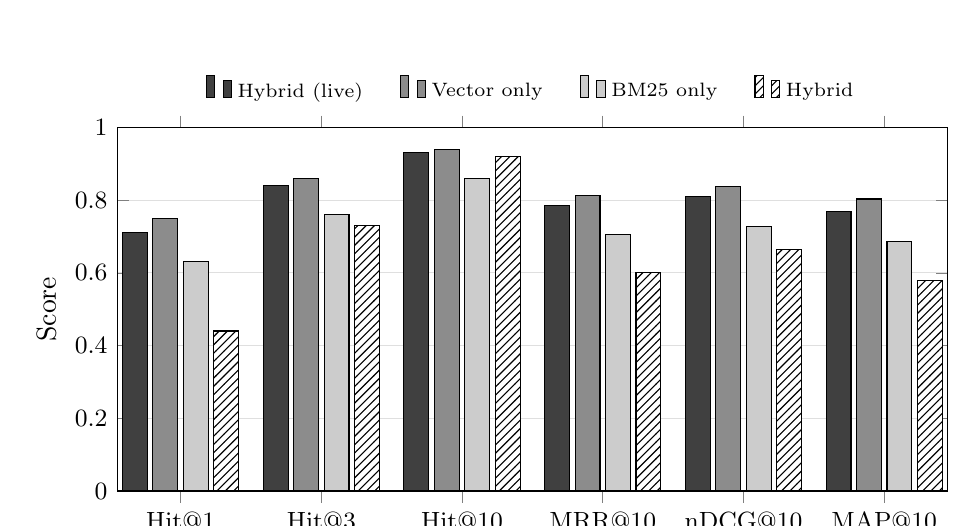
\begin{tikzpicture}
\begin{axis}[
  ybar, bar width=9pt, width=\textwidth, height=6.2cm,
  ymin=0, ymax=1, ylabel={Score},
  symbolic x coords={Hit@1,Hit@3,Hit@10,MRR@10,nDCG@10,MAP@10},
  xtick=data, tick label style={font=\small},
  legend style={font=\scriptsize, at={(0.5,1.04)}, anchor=south, legend columns=4, draw=none,
                /tikz/every even column/.append style={column sep=4mm}},
  enlarge x limits=0.09, ymajorgrids, grid style={gray!25},
]
\addplot[fill=black!75] coordinates {(Hit@1,0.71) (Hit@3,0.84) (Hit@10,0.93) (MRR@10,0.786) (nDCG@10,0.810) (MAP@10,0.768)};
\addplot[fill=black!45] coordinates {(Hit@1,0.75) (Hit@3,0.86) (Hit@10,0.94) (MRR@10,0.812) (nDCG@10,0.837) (MAP@10,0.803)};
\addplot[fill=black!20] coordinates {(Hit@1,0.63) (Hit@3,0.76) (Hit@10,0.86) (MRR@10,0.705) (nDCG@10,0.728) (MAP@10,0.687)};
\addplot[fill=white, postaction={pattern=north east lines}] coordinates {(Hit@1,0.44) (Hit@3,0.73) (Hit@10,0.92) (MRR@10,0.601) (nDCG@10,0.663) (MAP@10,0.578)};
\legend{Hybrid (live), Vector only, BM25 only, Hybrid, old bonus}
\end{axis}
\end{tikzpicture}
\caption{Quality metrics by configuration}
\label{fig:results-bars}
\end{figure}

No claim received an empty result list in any configuration. Hybrid search
took \textbf{76\,ms} at the median and \textbf{93\,ms} at the 95th
percentile, in-process on a laptop (network and sign-in checks excluded).

\subsection{Confidence}

\begin{table}[H]
\centering
\small
\begin{tabular}{lcc}
\toprule
\textbf{Configuration} & \textbf{Hit@1 (95\% CI)} & \textbf{MRR@10 (95\% CI)} \\
\midrule
Hybrid (live) & 0.62 -- 0.79 & 0.72 -- 0.85 \\
BM25 only & 0.54 -- 0.72 & 0.63 -- 0.78 \\
Vector only & 0.67 -- 0.83 & 0.75 -- 0.88 \\
Hybrid, old bonus & 0.34 -- 0.54 & 0.53 -- 0.68 \\
\bottomrule
\end{tabular}
\caption{Bootstrap 95\% intervals}
\label{tab:ci}
\end{table}

With 100 claims, a few lucky or unlucky ones move an average. The interval
of the old configuration does not overlap the live one's, so the
improvement is real. Hybrid and vector-only overlap almost completely, so the
gap between them may be chance.

\section{Finding: the Second-Chunk Bonus}
\label{sec:bonus}

Until this evaluation, a page scored its best chunk \emph{plus} 0.3 times its
second-best chunk, so that a page matching in two places would beat one
matching once. Under Reciprocal Rank Fusion, though, neighbouring ranks
score almost the same:

\[
\frac{1}{60+1} - \frac{1}{60+10} \approx 0.0021
\quad<\quad
0.3 \times \frac{1}{60+2} \approx 0.0048 .
\]

A single second match was therefore worth more than climbing nine places, and
\textbf{longer pages beat better matches}. When the old configuration put a
wrong abstract first, that abstract had 2.1 chunks on average; the right
answers had 1.3. A sweep of the bonus (Figure~\ref{fig:sweep}) showed every
non-zero value hurting, so the bonus was set to zero and pages are now
ranked by their best passage.

\begin{figure}[H]
\centering
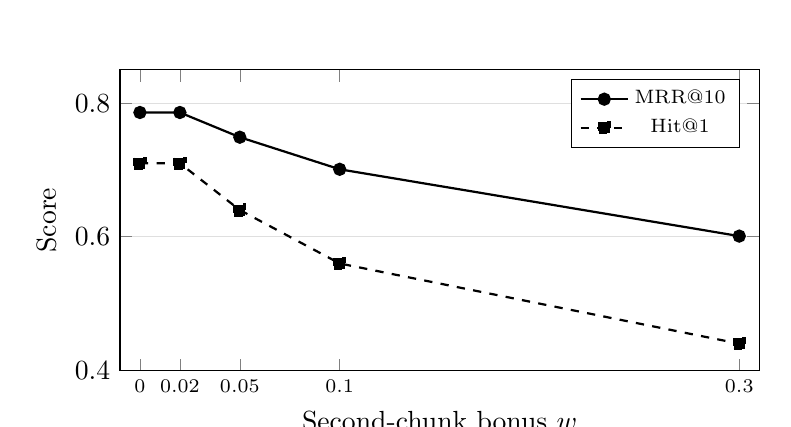
\begin{tikzpicture}
\begin{axis}[
  width=0.8\textwidth, height=5.4cm,
  xlabel={Second-chunk bonus $w$}, ylabel={Score},
  xmin=-0.01, xmax=0.31, ymin=0.4, ymax=0.85,
  xtick={0,0.02,0.05,0.1,0.3}, xticklabel style={font=\scriptsize, /pgf/number format/fixed},
  legend style={font=\scriptsize, at={(0.97,0.97)}, anchor=north east},
  ymajorgrids, grid style={gray!25}, mark size=2pt,
]
\addplot[thick, mark=*] coordinates {(0,0.786) (0.02,0.786) (0.05,0.749) (0.1,0.701) (0.3,0.601)};
\addplot[thick, dashed, mark=square*] coordinates {(0,0.71) (0.02,0.71) (0.05,0.64) (0.1,0.56) (0.3,0.44)};
\legend{MRR@10, Hit@1}
\end{axis}
\end{tikzpicture}
\caption{Effect of the second-chunk bonus on hybrid search}
\label{fig:sweep}
\end{figure}

\section{Other Findings}

\begin{itemize}
  \item \textbf{The relevance floor costs nothing on SciFact.} Removing it
  changed MRR@10 by 0.001 and left no claim without results; it removes
  weak vector-only matches, and the right abstract is rarely one of them. In
  real libraries it is what keeps unrelated pages off short result lists.
  \item \textbf{Hybrid and vector-only are level.} SciFact claims rarely
  share exact words with their abstracts, which favours meaning-based
  search. Hybrid is kept because everyday queries contain names, error
  messages, product codes and sites, which a vector-only search can miss.
  \item \textbf{BM25 gains as much as the others from page grouping.} BM25
  alone rose from MRR@10 0.41 with the bonus to 0.71 without it.
\end{itemize}

\section{Comparison with the Prototype}

\begin{table}[H]
\centering
\small
\begin{tabular}{llccc}
\toprule
\textbf{Version} & \textbf{Configuration} & \textbf{MRR@10} & \textbf{Recall@10} & \textbf{nDCG@10} \\
\midrule
\multirow{3}{*}{Prototype}
 & BM25 only & 0.648 & 0.812 & 0.678 \\
 & Vector only & 0.780 & 0.887 & 0.801 \\
 & Hybrid (min-max) & 0.754 & 0.917 & 0.789 \\
\midrule
\multirow{3}{*}{Final}
 & BM25 only & 0.705 & 0.837 & 0.728 \\
 & Vector only & \textbf{0.812} & \textbf{0.932} & \textbf{0.837} \\
 & Hybrid (RRF) & 0.786 & 0.922 & 0.810 \\
\bottomrule
\end{tabular}
\caption{Prototype and final system on SciFact}
\label{tab:proto-compare}
\end{table}

Every configuration of the final system beats its prototype counterpart on
every metric, the result of the stronger embedding model, smaller
overlapping chunks embedded with titles, rank fusion and best-passage page
scoring.

\section{Evaluation on a Personal Library}

SciFact measures scientific claims, not how people look for pages they have
read. A second evaluation runs on a real library with queries written by its
owner, each labelled \emph{navigational}, \emph{site}, \emph{topic} or
\emph{time}, and reports Recall@1/3/5/10 and MRR per category, with a
compare tool that lists every query whose rank changed. It was used to
measure site, time and URL understanding on a development library of 31
browsed pages among about 1{,}000 SciFact distractors:

\begin{table}[H]
\centering
\small
\begin{tabular}{lcccc}
\toprule
& \multicolumn{2}{c}{\textbf{Right page first}} & \multicolumn{2}{c}{\textbf{MRR}} \\
\cmidrule(lr){2-3}\cmidrule(lr){4-5}
\textbf{Query set} & before & after & before & after \\
\midrule
35 queries used while building & 0.86 & 0.94 & 0.900 & 0.971 \\
18 held-out queries & 0.72 & 0.94 & 0.787 & 0.944 \\
\bottomrule
\end{tabular}
\caption{Effect of site and time understanding on a personal library}
\label{tab:personal}
\end{table}

Most of the gain is in site queries (held-out MRR 0.75 $\rightarrow$ 1.00)
and time queries (0.38 $\rightarrow$ 1.00); topic-only queries are
unaffected, as intended. The sets are small, so the results indicate
direction rather than precise size.

% ==================================================
% CHAPTER 8: DEPLOYMENT AND OPERATIONS
% ==================================================

\chapter{Deployment and Operations}
\label{ch:deployment}

\section{Infrastructure}

MemoryLane runs on a single AWS EC2 \texttt{c7i-flex.large} instance (2 vCPU,
4\,GB RAM plus 2\,GB swap) in the Mumbai region, with an Elastic IP and the
domain \texttt{memorylane.site}. Three Docker Compose services make up the
system (Figure~\ref{fig:deployment}).

\begin{figure}[H]
\centering
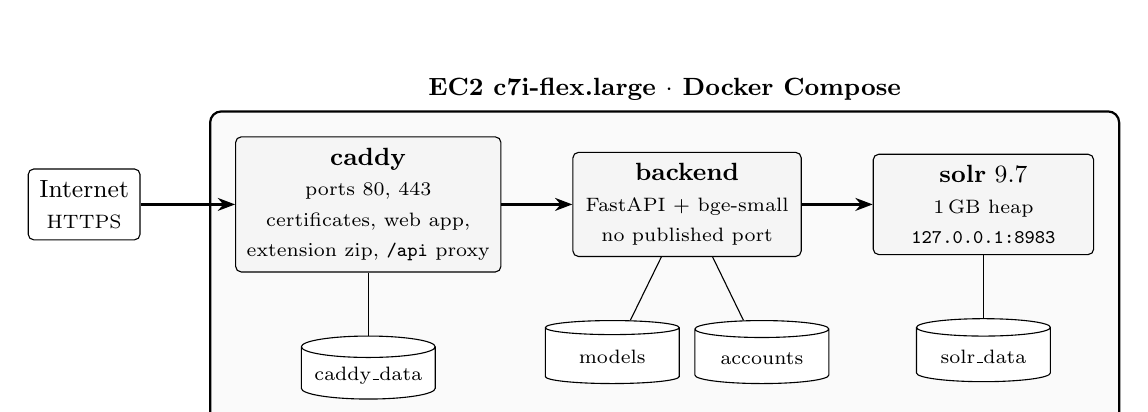
\begin{tikzpicture}[node distance=6mm and 10mm]
  \tikzset{vol/.style={db, minimum width=17mm, minimum height=8mm, font=\scriptsize, fill=white}}
  \node[comp, minimum width=31mm] (caddy) {\textbf{caddy}\\\scriptsize ports 80, 443\\\scriptsize certificates, web app,\\\scriptsize extension zip, \texttt{/api} proxy};
  \node[comp, right=9mm of caddy, minimum width=29mm] (backend) {\textbf{backend}\\\scriptsize FastAPI + bge-small\\\scriptsize no published port};
  \node[comp, right=9mm of backend, minimum width=28mm] (solr) {\textbf{solr} 9.7\\\scriptsize 1\,GB heap\\\scriptsize \texttt{127.0.0.1:8983}};
  \node[vol, below=8mm of caddy] (v1) {caddy\_data};
  \node[vol, below=8mm of backend, xshift=-9.5mm] (v2) {models};
  \node[vol, below=8mm of backend, xshift=9.5mm] (v3) {accounts};
  \node[vol, below=8mm of solr] (v4) {solr\_data};
  \draw[flow] (caddy) -- (backend);
  \draw[flow] (backend) -- (solr);
  \draw (caddy) -- (v1); \draw (backend) -- (v2); \draw (backend) -- (v3); \draw (solr) -- (v4);
  \begin{scope}[on background layer]
    \node[group, fill=gray!4, fit=(caddy)(solr)(v1)(v4), inner sep=9pt,
          label={[font=\small\bfseries]above:EC2 c7i-flex.large $\cdot$ Docker Compose}] (ec2) {};
  \end{scope}
  \node[box, left=12mm of caddy] (net) {Internet\\\scriptsize HTTPS};
  \draw[flow] (net) -- (caddy);
\end{tikzpicture}
\caption{Deployment: three containers and their volumes}
\label{fig:deployment}
\end{figure}

\begin{itemize}
  \item \textbf{Caddy} \cite{caddy} obtains and renews certificates
  automatically, redirects HTTP to HTTPS with HSTS, serves the built web app
  and the extension download, sets the Content Security Policy, and proxies
  \texttt{/api/*} to the backend.
  \item The Caddy image \emph{builds} the web app and zips the extension
  during \texttt{docker compose build}, so the files served always match the
  deployed code.
  \item Only ports 80 and 443 are open. The backend is reachable only
  through Caddy, and Solr listens on the server's localhost.
\end{itemize}

\section{Releasing a Change}

\begin{lstlisting}[language=bash]
cd ~/ucs503p-202627-MemoryLane && git pull origin master
cd code/src && docker compose up -d --build
docker compose logs -f backend
\end{lstlisting}

Schema changes are made first, by script, because Solr's automatic field
creation is off. Pages can be re-processed into a new core with the re-index
script, which never modifies the source core, and page vectors were
back-filled for older pages with a resumable script. Backups are EBS
snapshots of the instance's volume.

\section{Operations}

\begin{itemize}
  \item \textbf{Health}: \texttt{GET /api/health} reports Solr, the model and
  Gemini; Docker health checks restart unhealthy services, and every
  service restarts after a reboot.
  \item \textbf{Logs} are capped at three 10\,MB files per service and hold
  page ids, not URLs or queries.
  \item \textbf{Graceful degradation}: without Gemini, summaries are
  unavailable and everything else works; if email fails, reports wait in
  SQLite and are retried; if Cognito is unreachable, known sign-ins keep
  working.
  \item \textbf{Documentation} is published to GitHub Pages with MkDocs'
  \texttt{gh-deploy} command in strict mode, and the CI workflow checks the
  build on every change.
\end{itemize}

\section{Distribution of the Extension}

The extension is downloaded from the website as a zip built from the
deployed code and loaded unpacked in Chrome. Its version is bumped with
every change (2.4.2 at the time of writing), so users can see whether they
are up to date; the server's own checks protect against outdated
extensions in the meantime.

% ==================================================
% CHAPTER 9: CONCLUSION
% ==================================================

\chapter{Conclusion}
\label{ch:conclusion}

\section{Summary}

MemoryLane turns the pages a person reads into a memory they can search by
describing what they remember. Over the semester it grew from a local,
single-user prototype into a deployed, multi-user product: a Chrome extension
that saves pages and videos, with automatic capture that keeps only what was
read and looks like content; a cleaning, chunking and embedding pipeline; a
hybrid search that fuses BM25 and vector retrieval by rank, understands sites
and times in queries, filters weak matches and shows readable snippets; and a
web app with a library, undoable deletes, summaries and voice search, all
behind Cognito sign-in with isolation enforced in the data layer, and running
at \texttt{memorylane.site}.

\section{Achievements}

\begin{enumerate}
  \item \textbf{Retrieval quality}: on SciFact the live search puts the right
  abstract first for 71\% of claims and in the top ten for 93\%, with MRR@10
  0.786, ahead of the prototype on every metric.
  \item \textbf{Measurement that changed the product}: the expanded
  evaluation found a ranking defect that raised Hit@1 from 0.44 to 0.71 once
  fixed, a gain confirmed by non-overlapping confidence intervals.
  \item \textbf{Speed}: about 76\,ms per search at the median on modest
  hardware, with no GPU.
  \item \textbf{Security and privacy by construction}: per-user isolation in
  the Solr client, PKCE sign-in, verified-email account linking, privacy-safe
  logs, and automatic capture that refuses private pages twice.
  \item \textbf{Engineering discipline}: 551 automated tests, regression
  tests for every post-launch bug, eleven decision records, and a 48-page
  documentation site with its own meaning-based search.
\end{enumerate}

\section{Limitations}

\begin{itemize}
  \item \textbf{Benchmark scope}: SciFact is a scientific benchmark, and the
  personal-library evaluation used small query sets; neither fully
  represents everyday browsing.
  \item \textbf{Single server}: one instance is a single point of failure
  and caps throughput; the embedding model runs on the CPU in one process.
  \item \textbf{Capture coverage}: pages that render little text, videos
  without captions and content behind logins are saved poorly or not at all.
  \item \textbf{Server-side storage}: page text is stored on the server, and
  summaries send a page to an external model when asked; users must trust
  the operator.
  \item \textbf{Chrome only}: the extension targets Chromium browsers and is
  installed unpacked rather than from a store.
\end{itemize}

\section{Future Work}

\begin{enumerate}
  \item \textbf{Larger and broader evaluation}: more BEIR datasets and a
  larger personal query set, run automatically after every retrieval change.
  \item \textbf{Learned reranking}: enable the existing cross-encoder stage
  where memory allows, and measure it.
  \item \textbf{Summary fallback}: a second, cheaper model or an extractive
  summary when Gemini is unavailable.
  \item \textbf{Import}: bring in existing bookmarks and browser history.
  \item \textbf{Account features}: password change and signing out of every
  device from an account page.
  \item \textbf{Local-first mode}: on-device embedding and storage for users
  who do not want page text on a server.
  \item \textbf{Store distribution}: publish the extension in the Chrome Web
  Store, and port it to Firefox.
\end{enumerate}

\section{Final Remarks}

The prototype showed that content-based search over one's own reading was
possible. The final product shows that it can be made dependable, private
and fast enough to use every day, and that careful measurement matters as
much as new features: the largest single improvement of the semester came
from evaluating the system honestly and fixing what the numbers revealed.


% ==================================================
% BIBLIOGRAPHY AND APPENDICES
% ==================================================

\printbibliography[heading=bibintoc]

\appendix
% ==================================================
% APPENDICES
% ==================================================

\chapter{Search Configuration}
\label{app:config}

The search can be tuned without code changes through environment variables.
Table~\ref{tab:config} lists the retrieval and processing settings and the
values used in the live system and in the evaluation.

\begin{table}[H]
\centering
\small
\begin{tabularx}{\textwidth}{>{\ttfamily\raggedright\arraybackslash}p{0.33\textwidth} >{\ttfamily\raggedright\arraybackslash}p{0.23\textwidth} L}
\toprule
\textrm{\textbf{Setting}} & \textrm{\textbf{Value}} & \textbf{Meaning} \\
\midrule
EMBEDDING\_MODEL & bge-small-en-v1.5 & Sentence Transformers model (384-d) \\
DEFAULT\_CANDIDATE\_POOL & 50 & Chunks fetched from BM25 and from KNN \\
RRF\_K & 60 & Reciprocal Rank Fusion constant \\
BM25\_WEIGHT, VECTOR\_WEIGHT & 1.0, 1.0 & Weights of the two rankings \\
PAGE\_SECOND\_CHUNK\_WEIGHT & 0 & Bonus for a page's second chunk (off) \\
MIN\_VECTOR\_SIMILARITY & 0.55 & Cosine needed by meaning-only matches \\
KEYWORD\_FULL\_MATCH & 0.75 & Share of query words that keeps a keyword match \\
QUERY\_INTENT\_ENABLED & true & Site, time and URL understanding \\
RERANK\_ENABLED & false & Optional cross-encoder reranker \\
CHUNK\_MAX\_WORDS & 150 & Largest chunk \\
CHUNK\_OVERLAP\_WORDS & 30 & Words carried into the next chunk \\
CHUNK\_MIN\_WORDS & 40 & A shorter tail merges into the previous chunk \\
MAX\_PAGES\_PER\_USER & 5000 & Saved pages per account \\
\bottomrule
\end{tabularx}
\caption{Retrieval and processing settings}
\label{tab:config}
\end{table}

\chapter{Reproducing the Evaluation}
\label{app:reproduce}

The SciFact evaluation runs on any machine with Docker and the project's
Python environment, without touching the live server:

\begin{lstlisting}[language=bash]
docker run -d --name ml-eval-solr -p 127.0.0.1:8983:8983 solr:9.7
docker exec ml-eval-solr solr create -c memorylane_eval -d _default
CORE_NAME=memorylane_eval ./scripts/setup_solr.sh
python -m evaluation.scifact_ingest   --solr-base http://localhost:8983/solr
python -m evaluation.scifact_evaluate --solr-base http://localhost:8983/solr
docker rm -f ml-eval-solr
\end{lstlisting}

Indexing takes about two minutes and the five-configuration evaluation about
three. The report, \texttt{evaluation/scifact\_report.json}, records the
settings used, every metric with its confidence interval, and the rank of
the first relevant result for each claim.

\chapter{Project Resources}
\label{app:resources}

\begin{table}[H]
\centering
\small
\begin{tabularx}{\textwidth}{p{0.25\textwidth} L}
\toprule
\textbf{Resource} & \textbf{Location} \\
\midrule
Live application & \url{https://memorylane.site} \\
Documentation & \url{https://rabeeh18.github.io/ucs503p-202627-MemoryLane/} \\
Source code & \url{https://github.com/rabeeh18/ucs503p-202627-MemoryLane} \\
Extension & \url{https://memorylane.site/memorylane-extension.zip} \\
\bottomrule
\end{tabularx}
\caption{Project resources}
\label{tab:resources}
\end{table}


\end{document}
